\chapter{Graphen}

In Graphen verbinden Kanten Knoten.
Anwendung von Graphen.


Kürzeste Wege.
Straßen

\begin{figure}
    \centering
    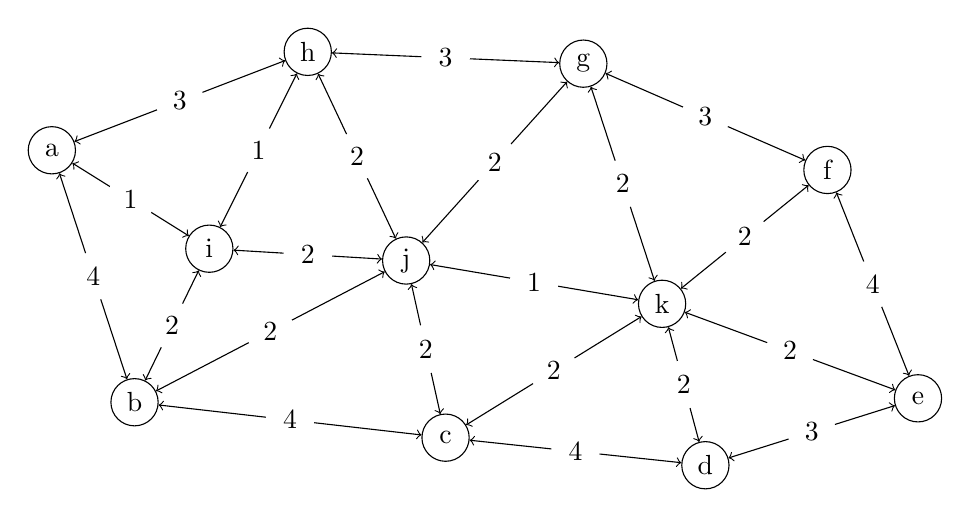
\begin{tikzpicture}
        % Nodes
        \node[circle, draw, minimum size=0.6cm, inner sep=0pt] at (0.5* 0.0, 0.5* 8.5)  (a)    {a};
        \node[circle, draw, minimum size=0.6cm, inner sep=0pt] at (0.5* 2.1, 0.5* 2.1)  (b)    {b};
        \node[circle, draw, minimum size=0.6cm, inner sep=0pt] at (0.5* 10.0, 0.5* 1.2)  (c)    {c};
        \node[circle, draw, minimum size=0.6cm, inner sep=0pt] at (0.5* 16.6, 0.5* 0.5)  (d)    {d};
        \node[circle, draw, minimum size=0.6cm, inner sep=0pt] at (0.5* 22.0, 0.5* 2.2)  (e)    {e};
        \node[circle, draw, minimum size=0.6cm, inner sep=0pt] at (0.5* 19.7, 0.5* 8.0)  (f)    {f};
        \node[circle, draw, minimum size=0.6cm, inner sep=0pt] at (0.5* 13.5, 0.5* 10.7)  (g)    {g};
        \node[circle, draw, minimum size=0.6cm, inner sep=0pt] at (0.5* 6.5, 0.5* 11.0)  (h)    {h};
        \node[circle, draw, minimum size=0.6cm, inner sep=0pt] at (0.5* 4.0, 0.5* 6.0)  (i)    {i};
        \node[circle, draw, minimum size=0.6cm, inner sep=0pt] at (0.5* 9.0, 0.5* 5.7)  (j)    {j};
        \node[circle, draw, minimum size=0.6cm, inner sep=0pt] at (0.5* 15.5, 0.5* 4.6)  (k)    {k};


        \draw[<->]  (a) edge node[circle, fill=white] {4} (b);
        \draw[<->]  (a) edge node[circle, fill=white] {3} (h);
        \draw[<->]  (a) edge node[circle, fill=white] {1} (i);

        \draw[<->]  (b) edge node[circle, fill=white] {4} (c);
        \draw[<->]  (b) edge node[circle, fill=white] {2} (i);
        \draw[<->]  (b) edge node[circle, fill=white] {2} (j);

        \draw[<->]  (c) edge node[circle, fill=white] {4} (d);
        \draw[<->]  (c) edge node[circle, fill=white] {2} (j);
        \draw[<->]  (c) edge node[circle, fill=white] {2} (k);

        \draw[<->]  (d) edge node[circle, fill=white] {3} (e);
        \draw[<->]  (d) edge node[circle, fill=white] {2} (k);

        \draw[<->]  (e) edge node[circle, fill=white] {4} (f);
        \draw[<->]  (e) edge node[circle, fill=white] {2} (k);

        \draw[<->]  (f) edge node[circle, fill=white] {3} (g);
        \draw[<->]  (f) edge node[circle, fill=white] {2} (k);

        \draw[<->]  (g) edge node[circle, fill=white] {3} (h);
        \draw[<->]  (g) edge node[circle, fill=white] {2} (j);
        \draw[<->]  (g) edge node[circle, fill=white] {2} (k);

        \draw[<->]  (h) edge node[circle, fill=white] {1} (i);
        \draw[<->]  (h) edge node[circle, fill=white] {2} (j);

        \draw[<->]  (i) edge node[circle, fill=white] {2} (j);

        \draw[<->]  (j) edge node[circle, fill=white] {1} (k);
    \end{tikzpicture}
    \caption{Beispielgraph}
\end{figure}

\todo{Graphen auf Kinderniveau erklären und schöne Bilder von Graphen zeigen}.

\section{Definitionen}
Damit in den nachfolgenden Kapiteln sinnvoll argumentiert werden kann, ist es notwendig, einige Begriffe zu definieren.

\begin{definition}[Graph]
    Sofern nicht anders angegeben, wird ein endlicher, gerichteter Graph mit Kantengewichten, ohne Mehrfachkanten und Schleifen, einfach als Graph bezeichnet.

    Als Schreibweise wird $G = (V, E)$ verwendet, wobei $V$ die Knotenmenge und $E$ die Kantenmenge ist. Eine Kante ist ein Tupel $(t, h, w)$. $t \in V$ wird als \emph{Fuß}, $h \in V$ als \emph{Kopf} und $w \in \mathbb{R}$ als \emph{Gewicht} bezeichnet. Gelegentlich wird auch nur $(t, h)$ geschrieben, um auszudrücken, dass zwei Knoten verbunden sind. Da ein Graph keine Mehrfachkanten zulässt, definiert diese Schreibweise auch eindeutig das Kantengewicht.

    Wird $G$ als ungerichtet bezeichnet, dann gilt $(t, h) \in E \Leftrightarrow (h, t) \in E$.
\end{definition}

In einem Graphen gibt es oft das Interesse, von einem Knoten zu einem anderen zu gelangen.
Diese Verbindungen zwischen Knoten werden durch sogenannte Wege dargestellt.

\begin{definition}[Weg]
    Ein Weg auf einem Graph $G = (V, E)$ ist eine Folge von Knoten $v_1, \dotsc, v_n$, für die gilt, dass benachbarte Knoten im Weg eine Kante in $E$ bilden.

    \todo{Wie nenne ich die Hoplänge?}

    Die Summe der Kantengewichte aller Kanten $(v_i, v_{i + 1})$ wird \emph{Länge} des Weges genannt. Der Knoten $v_1$ wird Startknoten, $v_n$ Zielknoten genannt.
\end{definition}

Zwischen zwei Knoten kann es mehrere unterschiedliche Wege geben.
Diese Wege können auch unterschiedliche Länge haben.

\begin{definition}[Kürzester Weg]
    Ein Weg $v_1, \dotsc, v_n$ ist \emph{ein kürzester Weg}, wenn die Länge des Weges unter allen Wegen von $v_1$ nach $v_n$ minimal ist. Die Länge des kürzesten Weges wird als \emph{Abstand} von $v_1$ und $v_n$ bezeichnet. Die Definition des Graphen lässt es zu, dass es mehrere kürzeste Wege zwischen zwei Knoten gibt.

    Sei $P \subset V \times V$ die Menge der Knoten, zwischen denen ein Weg existiert. Dann sind definiert:
    \begin{enumerate}
        \item
              ${spd} \colon P \to \mathbb{R}$ weist einem Knotenpaar den Abstand zu.

        \item
              ${sp} \colon P \to V \times V \times \dots \times V$ weist einem Knotenpaar einen kürzesten Weg zu.
    \end{enumerate}
\end{definition}

\begin{definition}[Umkehrgraph]
    Sei $G = (V, E)$ ein Graph. Dann ist $G^T = (V, E^T)$ mit $(t, h, w) \in E \Leftrightarrow (h, t, w) \in E^T$ der \emph{Umkehrgraph} von $G$.
\end{definition}

Zusätlich zum finden eines Weges zwischen zwei Knoten ist es häufig notwendig den kürzesten Weg von einem Knoten zu allen anderen Knoten zu finden.
Auch die Umkehrung dieses Problem ist interesannt, also die kürzesten Wege von allen Knoten zu einem zu bestimmen.
Diese Probleme sind äuivalent, da das Finden alle kürzesten Wege zu einem Knoten auf einem Graph $G$ dem Finden aller kürzester Wege auf dem Umkehrgraph $G^T$ entspricht.

\section{Nicht-Straßen Graphen}

Straßengraphen haben eine Hierarische Struktur.
Fahren von A nach B führt auf immer schneller Straßen bis zu einem gewissen Punkt, dann immer langsamere Straßen.
Diese Eigenschaft lässt sich für das Wegfinden ausnutzen.
Diese Eigenscahft zu benenne ist nicht so leicht.
Hier vielleicht die Highway Dimension erklären.

Sonstige Metriken interesannt?
Wie kann ich einen gegebenen Graph klassifizieren, ob er "teuer" zum suchen ist?

Die vis Graphen haben zwar viele Kanten aber es werden selten Knoten mehrfach gepusht.

Kürzeste Pfad Queries mit dem klassischen Dijksta Algorithmus sind auf den visibility Graphen deutlich teuerer als auf den triangulierten Graphen.



\section{Dijkstra Algorithmus}

Als Baseline für das suchen verwende ich Dijkstra.
Später wird der Algorithmus auch benutzt werden.
Um die Kosten einer Suche nicht nur in Zeit auszudrücken wird noch definiert:
Die Mächtigkeit der Menge $u$ als Dijkstra Rank
Die Anzahl der Operationen \ref{graphs:dijkstra:pop} quqe pops.


\todo{Dijkstra Algorithmus erklären und Dijkstra Paper zitieren}

\begin{algorithm}
    \caption{Dijkstra Algorithmus}
    \begin{algorithmic}[1]
        \Require Graph $G = (V, E)$, Startknoten $s \in V$, Zielknoten $t \in V$
        \Ensure ${dist}$, ${pre}$
        \State // Initialisiere Distanz- und Vorgänger-Funktion
        \ForAll{$v \in V$}
        \State ${dist}(v) \leftarrow \infty$
        \State ${pre}(v) \leftarrow {none}$
        \EndFor


        \State
        \State // Initialisiere Vorrangwarteschlange
        \State ${dist}(s) \leftarrow 0$
        \State $Q\leftarrow \{ s \}$

        \State
        \While{$Q \neq \emptyset$}
        \State $u \leftarrow{extract\_min}(Q)$\label{graphs:dijkstra:pop}

        \State
        \State // Beende frühzeitig wenn Zielknoten gefunden wurde
        \If {$u = t$}
        \State \textbf{break}
        \EndIf

        \State
        \State // Aktualisiere Nachbarn
        \ForAll{$(u, v, w) \in E$}
        \If {${dist}(u) + w < {dist}(v)$}
        \State ${dist}(v) \leftarrow {dist}(u) + w$
        \State ${pre}(u) \leftarrow v$
        \State $Q = Q \cup \{ v \}$
        \EndIf
        \EndFor

        \EndWhile

        \State
        \State \Return ${dist}$, ${pre}$
    \end{algorithmic}
\end{algorithm}


\section{Datenstrukturen}

Vertices sind natürliche Zahlen bzw uint32.
Ein Graph enthält idealerweise keine isolierten Knoten.
isolierte Knoten sind doof für dijkstra und co.
Die Menge der Knoten ist definiert durch Ihre Anzahl.
Gibt es $n \in \mathbb{N}$ Knoten, so sind es $0, \dotsc, n - 1$.

Ein Graph der diese Eigenschaft nicht erfüllt, kann durch eine Mapping der Knoten in die Form gebracht werden
Hierfür wurde ein python script geschrieben
\todo{Vergleiche degree histogramme}

Jenachdem was mit dem Graph gemacht werden soll, sind verschiedene Eigenschaften von Vorteil.
Manchmal ist eine effiziente Nachbar Abfrage wichtig,
Manchmal das bearbeiten des Graphes, einfügen oder löschen von Knoten

Es wurde ein dyn Trait benutzt, welches eine Overhead hat und kein inlining zulässt.
Dafür lassen sich verschiedene Methoden vergleichen.

Die Grundlegenden Implementierungen kennen nur ihre Vorgänger.
Ein Reversibe Graph besteht aus einem Graph und seinem Umkehrgraph.
Gleiche Datenstruktur.

\subsection{VecVecGraph}
Mäßig schnelle Queries
Einfügen mit suche.
Bei vielen Knoten teuer.

\subsection{VecHashMap}
Besser Indexmap???

Eher langsame Queries.
Einfügen in O(1).

\subsection{VecGraph}
Schnelle Querries.
Einfügen sehr teuer.


\section{Archivierung}

Zum Speichern von Graphen wird textbasierter Format benutzt, welches die Dateiendung \emph{.fmi} nutzt.
Es ist wie folgt definiert:
\begin{definition}[FMI Dateiformat]
    Eine Datei des Dateiformates FMI besteht aus den folgenden Zeilen (in Ordnung der Auflistung)
    \begin{enumerate}
        \item
              Beliebig viele Kommentarzeilen die mit \# beginnnen

        \item
              Eine leere Zeilen

        \item
              Anzahl der Knoten

        \item
              Anzahl der Kanten

        \item
              Knoten mit nodeID nodeID2 latitude longitude elevation

        \item
              Kanten mit srcIDX trgIDX cost type maxspeed
    \end{enumerate}
\end{definition}

Die Bereitgestellten Dateien sind noch zu reinigen.
Sie enthalten isolierten Knoten.
Die Kantengewichte der Sichtbarkeitsgraphen sind float.
Meine Implementation rechnet mit uint32.

Dafür habe ich ein python script geschrieben.
Es wird jeweils ein vis und graph Paar zusammen bearbeitet.
Es entfernt isolierte Knoten und rundet die Kantengewichte auf (damit keine 0 Kanten entstehen).
Die Triangulierten Graphen enthalten jeweils 4 Kanten (2 ungerichtete) mit einem Kantengewicht von 0.
Diese Kanten wurden beibehalten.

\todo{Plot degree before after}